\documentclass[11pt,a4paper]{article}
\usepackage[utf8]{inputenc}
\usepackage[T1]{fontenc}
\usepackage[english]{babel}
\usepackage[margin=2cm]{geometry}
\usepackage{amsmath,amssymb}
\usepackage{graphicx}
\usepackage{float}
\usepackage{booktabs}
\usepackage{xcolor}
\usepackage[title]{appendix}
\usepackage{hyperref}
\graphicspath{{graphs/}}
% Sample period written by Stata in graphs/smp_*.tex (n.a. if the file does not exist yet)
\newcommand{\smp}[1]{\IfFileExists{graphs/smp_#1.tex}{\input{graphs/smp_#1.tex}\unskip}{n.a.}}
% Text to be written once the results have been read
\newcommand{\tbc}[1]{\textcolor{red}{[TO BE COMPLETED: #1]}}

\title{Energy price shocks, prices and wages in the euro area: graphs}
\date{\today}

\begin{document}
\maketitle
\tableofcontents
\clearpage

%==============================================================================
\section{Data and specification}
%==============================================================================

\subsection{Variables}

\begin{table}[H]
\centering
\footnotesize
\begin{tabular}{llp{6.2cm}l}
\toprule
Symbol & Variable & Definition & Source \\
\midrule
\multicolumn{4}{l}{\emph{Price change} $s_{t}$ (year-on-year \% change of the quarterly average, divided by 10)} \\
 & \texttt{OilSpotUSDBarrel} & Oil spot price, USD per barrel & \texttt{Data\_OIL\_ELE\_GAS.xlsx} \\
 & \texttt{TTFSpotEURMWH} & TTF natural gas spot price, EUR/MWh & \texttt{Data\_OIL\_ELE\_GAS.xlsx} \\
 & \texttt{ELEEURMWH} & Wholesale electricity price, EUR/MWh, by country (OLS only) & \texttt{Data\_OIL\_ELE\_GAS.xlsx} \\
\midrule
\multicolumn{4}{l}{\emph{Instruments} $z_{k,t}$, $k=1,2,3$ (monthly shock in the $k$-th month of quarter $t$)} \\
 & \texttt{oilMP1}--\texttt{3} & Oil supply news shock (for the oil price) & Mori and Peersman \\
 & \texttt{gasAG1}--\texttt{3} & Gas supply shock (for the gas price) & Alessandri and Gazzani (2025) \\
\midrule
\multicolumn{4}{l}{\emph{Outcome} $y_{t}$} \\
 & \texttt{hicp} & HICP, all items, year-on-year \% change & Eurostat \\
 & \texttt{contr} & Negotiated wages (INWR), total economy, year-on-year \% change & ECB \\
 & \texttt{wageH} & Gross wages per hour worked, year-on-year \% change & Eurostat, quarterly NA \\
 & \texttt{occH} & Hours worked, total economy, quarter-on-quarter \% change & Eurostat, quarterly NA \\
 & \texttt{dur} & Unemployment rate, quarter-on-quarter change (percentage points) & Eurostat \\
\midrule
\multicolumn{4}{l}{\emph{Controls} $x_{t}$ (as in Corsello and Foschi, 2026; without \texttt{ur} for \texttt{dur})} \\
 & \texttt{lip} & Log industrial production (B--D, seasonally adjusted) & Eurostat \\
 & \texttt{ur} & Unemployment rate (seasonally adjusted, \% of labour force) & Eurostat \\
 & \texttt{bund1y} & 1-year Bund yield (common to all countries) & Bundesbank \\
$C_t$ & \texttt{dcovid} & Dummy 2020q1--2022q4 & \\
\bottomrule
\end{tabular}
\end{table}

\noindent Quarterly frequency (monthly series are averages over complete quarters);
horizon $h = 0,\dots,12$ quarters; $p = 4$ lags; time series for the euro area (EA)
and for DE, IT, NL, ES, FR, BE. Main text: IV responses to oil and gas in the same
graph, for the euro area and for the euro area with the individual countries
(consumer prices, negotiated wages, hourly wages). Appendix: IV responses of hours
worked and of the unemployment rate; IV robustness; OLS estimates for comparison,
including electricity, for which no instrument is available.

\subsection{IV local projections}

\noindent The year-on-year change of the oil (gas) price $s_t$ is instrumented with the
monthly oil (gas) supply shocks. The instruments are monthly and the projections
quarterly: the three monthly shocks of quarter $t$, $z_{1,t}, z_{2,t}, z_{3,t}$, enter
as separate instruments (unrestricted MIDAS; Foroni, Marcellino and Schumacher, 2015),
so that the first stage estimates how much each month moves the quarterly average
price, conditional on all controls. Two-stage least squares, one regression per
country and horizon (Newey--West standard errors with $h+1$ lags):
\begin{align}
s_{t} &= c^h + \sum_{k=1}^{3} g_k^h z_{k,t}
 + \sum_{l=1}^{p} \left( \gamma_l^h y_{t-l} + \delta_l^h s_{t-l} + \phi_l^{h\prime} x_{t-l} \right)
 + \kappa^h C_t + u_{t} \\
y_{t+h} &= \alpha^h + \beta^h \hat s_{t}
 + \sum_{l=1}^{p} \left( \tilde\gamma_l^h y_{t-l} + \tilde\delta_l^h s_{t-l} + \tilde\phi_l^{h\prime} x_{t-l} \right)
 + \tilde\kappa^h C_t + \varepsilon_{t+h}
\end{align}
$\beta^h$ is the response of $y$ at horizon $h$ to a 10 percentage point increase in
the year-on-year growth of the price. Shock dates $t$ require the instruments; the
outcome $y_{t+h}$ can extend beyond their end. The strength of the first stage is
measured by the effective $F$ statistic of Montiel Olea and Pflueger (2013), robust
to heteroskedasticity and autocorrelation, against the critical value for a maximum
2SLS bias of 10\% (reported in the log of \texttt{an\_lpiv\_energy\_ea.do}).

\noindent Graphs: $\hat\beta^h$ for $h=0,\dots,12$, 90\% confidence bands.

\subsection{Robustness}

\noindent For the euro area: (i) quarterly-average instrument, one instrument equal to the
average of the three monthly shocks; (ii) pre-COVID sample, data before 2020q1 only
($t+h \le$ 2019q4), without $C_t$.

\subsection{OLS local projections (Appendix~\ref{app:ols})}

\noindent Same specification estimated by OLS, with $s_t$ not instrumented (time series;
for electricity, a panel with country fixed effects, employment weights and
Driscoll--Kraay standard errors):
\begin{equation}
y_{t+h} = \alpha^h + \beta^h s_{t}
 + \sum_{l=1}^{p} \left( \gamma_l^h y_{t-l} + \delta_l^h s_{t-l} + \phi_l^{h\prime} x_{t-l} \right)
 + \kappa^h C_t + \varepsilon_{t+h}
\end{equation}

\subsection{Sources}

\begin{itemize}
\item HICP: Eurostat, \texttt{prc\_hicp\_midx} (\texttt{CP00}, index 2015=100). Core inflation
 (\texttt{TOT\_X\_NRG\_FOOD}) is downloaded and kept in the dataset but not used in the estimates.
\item Negotiated wages: ECB, indicator of negotiated wage rates (INW), total economy,
 annual growth rates; national source series for DE and FR.
\item Wages, hours worked, employment: Eurostat, quarterly national accounts.
\item Industrial production: Eurostat, \texttt{sts\_inpr\_m} (B--D, seasonally adjusted, 2021=100).
 Unemployment rate: Eurostat, \texttt{une\_rt\_m} (seasonally adjusted, total).
\item 1-year Bund yield: Deutsche Bundesbank, term structure of listed Federal securities
 (Svensson method, residual maturity 1 year), series
 \texttt{BBSIS.M.I.ZST.ZI.EUR.S1311.B.A604.R01XX.R.A.A.\_Z.\_Z.A}.
\item Instruments: oil supply news shock of Mori and Peersman (column ``Updated sample
 2025m12'' of the authors' spreadsheet); gas supply shock of Alessandri and Gazzani
 (2025), \emph{Journal of Monetary Economics} 151, 103749 (file \texttt{GasSupplyShocks.xlsx},
 sheet \texttt{2025update}).
\item Energy prices: file \texttt{Data\_OIL\_ELE\_GAS.xlsx} (monthly data).
\end{itemize}

\clearpage
%==============================================================================
\section{IV responses to oil and gas price shocks}
%==============================================================================

\subsection{Consumer prices}

\noindent\textbf{Comment.} \tbc{reading of the IV responses of HICP to oil and gas price shocks: sign, size, timing and persistence; differences between oil and gas and across countries; comparison with OLS (Appendix~\ref{app:ols})}.


\begin{figure}[H]
  \centering
  \caption{Oil and gas $\rightarrow$ HICP: euro area}
  \label{fig:lp_iv_og_EA_hicp}
  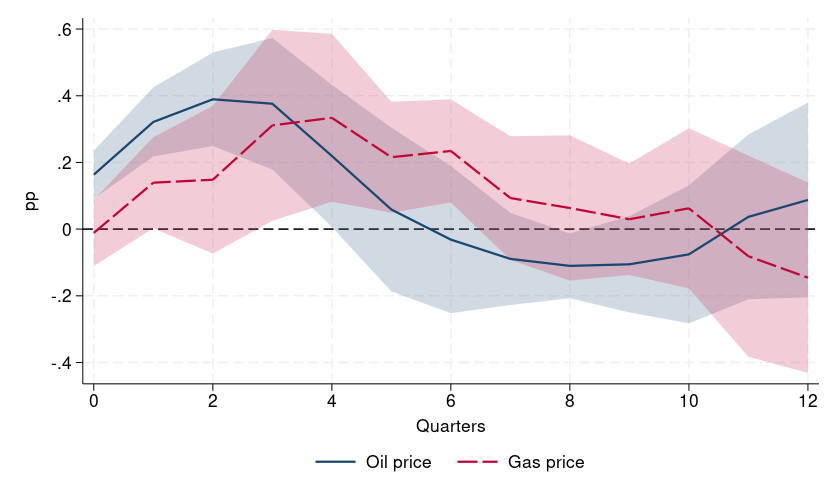
\includegraphics[width=0.7\textwidth]{lp_iv_og_EA_hicp.png}
  \begin{minipage}{0.95\textwidth}\footnotesize
  \emph{Notes}: Response (percentage points) of year-on-year HICP inflation to a 10 percentage point increase in the year-on-year growth of the oil and natural gas prices; 90\% confidence bands. 2SLS local projections: the oil price change is instrumented with the three monthly Mori--Peersman oil supply news shocks of the quarter, the gas price change with the three monthly Alessandri--Gazzani gas supply shocks of the quarter. Time-series estimate for the euro area, Newey--West standard errors. Controls (both stages): 4 lags of the outcome and of the price change, log industrial production, unemployment rate and 1-year Bund yield; COVID dummy 2020--2022. Sample (shock dates, $h=0$): \smp{lp_iv_og_EA_hicp}. Sources: Eurostat (HICP, \texttt{prc\_hicp\_midx}); Instruments: Mori and Peersman; Alessandri and Gazzani (2025). Eurostat and Bundesbank for the controls. Energy prices: quarterly averages of monthly data (file \texttt{Data\_OIL\_ELE\_GAS.xlsx}).
  \end{minipage}
\end{figure}

\begin{figure}[H]
  \centering
  \caption{Oil and gas $\rightarrow$ HICP: euro area and countries}
  \label{fig:lp_iv_og_ctry_hicp}
  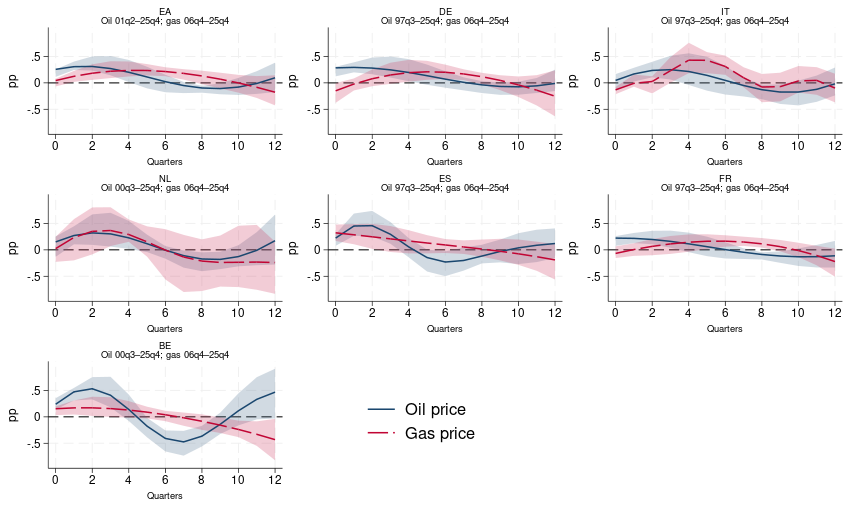
\includegraphics[width=1\textwidth]{lp_iv_og_ctry_hicp.png}
  \begin{minipage}{0.95\textwidth}\footnotesize
  \emph{Notes}: Response (percentage points) of year-on-year HICP inflation to a 10 percentage point increase in the year-on-year growth of the oil and natural gas prices; 90\% confidence bands. 2SLS local projections: the oil price change is instrumented with the three monthly Mori--Peersman oil supply news shocks of the quarter, the gas price change with the three monthly Alessandri--Gazzani gas supply shocks of the quarter. Time series for the euro area and for each country, Newey--West standard errors; same vertical scale in all panels; the sample (shock dates, $h=0$) for oil and gas is shown under each panel name. Controls (both stages): 4 lags of the outcome and of the price change, log industrial production, unemployment rate and 1-year Bund yield; COVID dummy 2020--2022. Sources: Eurostat (HICP, \texttt{prc\_hicp\_midx}); Instruments: Mori and Peersman; Alessandri and Gazzani (2025). Eurostat and Bundesbank for the controls. Energy prices: quarterly averages of monthly data (file \texttt{Data\_OIL\_ELE\_GAS.xlsx}).
  \end{minipage}
\end{figure}

\clearpage

\subsection{Negotiated wages}

\noindent\textbf{Comment.} \tbc{reading of the IV responses of negotiated wages to oil and gas price shocks: sign, size, timing and persistence; differences between oil and gas and across countries; comparison with OLS (Appendix~\ref{app:ols})}.


\begin{figure}[H]
  \centering
  \caption{Oil and gas $\rightarrow$ negotiated wages: euro area}
  \label{fig:lp_iv_og_EA_contr}
  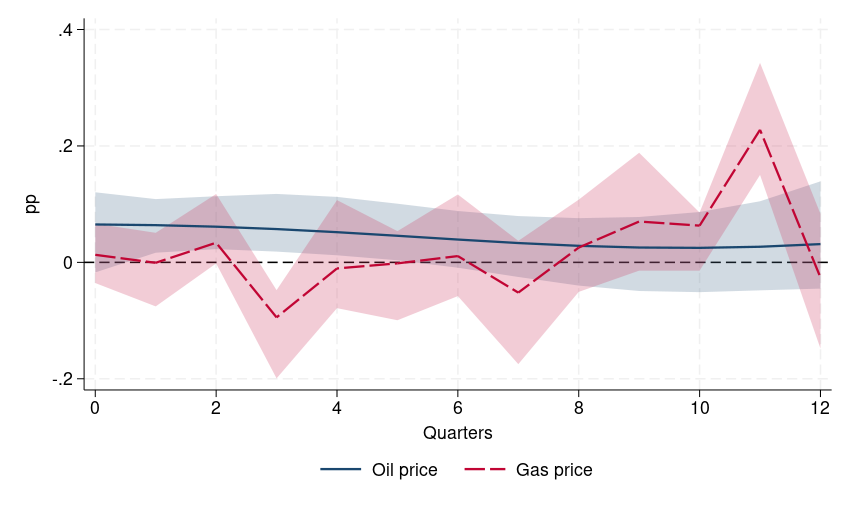
\includegraphics[width=0.7\textwidth]{lp_iv_og_EA_contr.png}
  \begin{minipage}{0.95\textwidth}\footnotesize
  \emph{Notes}: Response (percentage points) of year-on-year negotiated wage growth to a 10 percentage point increase in the year-on-year growth of the oil and natural gas prices; 90\% confidence bands. 2SLS local projections: the oil price change is instrumented with the three monthly Mori--Peersman oil supply news shocks of the quarter, the gas price change with the three monthly Alessandri--Gazzani gas supply shocks of the quarter. Time-series estimate for the euro area, Newey--West standard errors. Controls (both stages): 4 lags of the outcome and of the price change, log industrial production, unemployment rate and 1-year Bund yield; COVID dummy 2020--2022. Sample (shock dates, $h=0$): \smp{lp_iv_og_EA_contr}. Sources: ECB (indicator of negotiated wage rates, INW); Instruments: Mori and Peersman; Alessandri and Gazzani (2025). Eurostat and Bundesbank for the controls. Energy prices: quarterly averages of monthly data (file \texttt{Data\_OIL\_ELE\_GAS.xlsx}).
  \end{minipage}
\end{figure}

\begin{figure}[H]
  \centering
  \caption{Oil and gas $\rightarrow$ negotiated wages: euro area and countries}
  \label{fig:lp_iv_og_ctry_contr}
  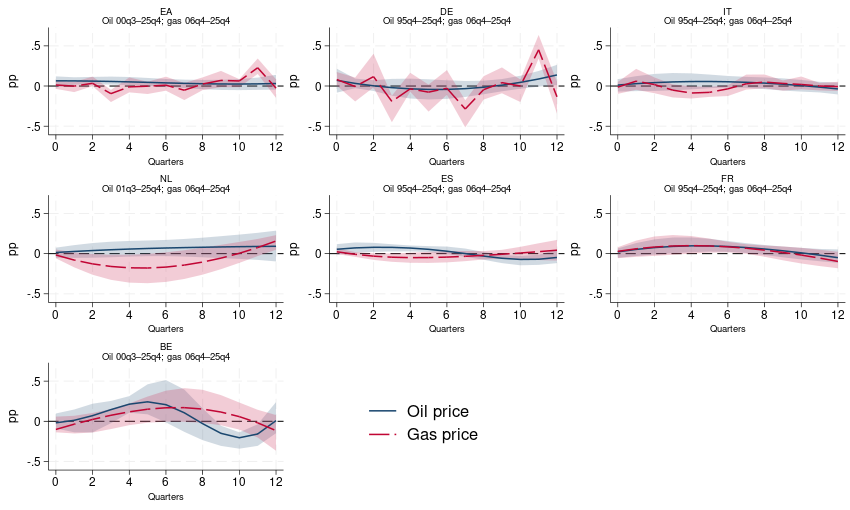
\includegraphics[width=1\textwidth]{lp_iv_og_ctry_contr.png}
  \begin{minipage}{0.95\textwidth}\footnotesize
  \emph{Notes}: Response (percentage points) of year-on-year negotiated wage growth to a 10 percentage point increase in the year-on-year growth of the oil and natural gas prices; 90\% confidence bands. 2SLS local projections: the oil price change is instrumented with the three monthly Mori--Peersman oil supply news shocks of the quarter, the gas price change with the three monthly Alessandri--Gazzani gas supply shocks of the quarter. Time series for the euro area and for each country, Newey--West standard errors; same vertical scale in all panels; the sample (shock dates, $h=0$) for oil and gas is shown under each panel name. Controls (both stages): 4 lags of the outcome and of the price change, log industrial production, unemployment rate and 1-year Bund yield; COVID dummy 2020--2022. Sources: ECB (indicator of negotiated wage rates, INW); Instruments: Mori and Peersman; Alessandri and Gazzani (2025). Eurostat and Bundesbank for the controls. Energy prices: quarterly averages of monthly data (file \texttt{Data\_OIL\_ELE\_GAS.xlsx}).
  \end{minipage}
\end{figure}

\clearpage

\subsection{National accounts wages}

\noindent\textbf{Comment.} \tbc{reading of the IV responses of hourly wages to oil and gas price shocks: sign, size, timing and persistence; differences between oil and gas and across countries; comparison with OLS (Appendix~\ref{app:ols})}.


\begin{figure}[H]
  \centering
  \caption{Oil and gas $\rightarrow$ hourly wages: euro area}
  \label{fig:lp_iv_og_EA_wageH}
  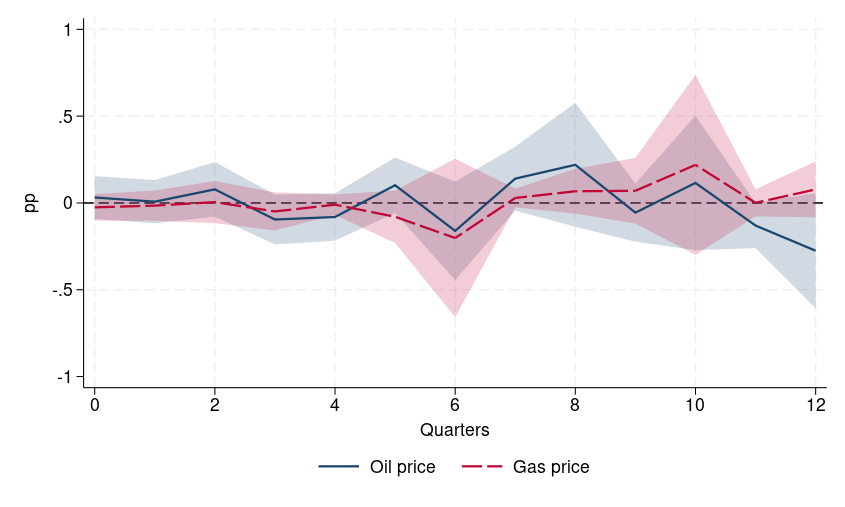
\includegraphics[width=0.7\textwidth]{lp_iv_og_EA_wageH.png}
  \begin{minipage}{0.95\textwidth}\footnotesize
  \emph{Notes}: Response (percentage points) of year-on-year growth in gross wages per hour worked to a 10 percentage point increase in the year-on-year growth of the oil and natural gas prices; 90\% confidence bands. 2SLS local projections: the oil price change is instrumented with the three monthly Mori--Peersman oil supply news shocks of the quarter, the gas price change with the three monthly Alessandri--Gazzani gas supply shocks of the quarter. Time-series estimate for the euro area, Newey--West standard errors. Controls (both stages): 4 lags of the outcome and of the price change, log industrial production, unemployment rate and 1-year Bund yield; COVID dummy 2020--2022. Sample (shock dates, $h=0$): \smp{lp_iv_og_EA_wageH}. Sources: Eurostat (quarterly national accounts); Instruments: Mori and Peersman; Alessandri and Gazzani (2025). Eurostat and Bundesbank for the controls. Energy prices: quarterly averages of monthly data (file \texttt{Data\_OIL\_ELE\_GAS.xlsx}).
  \end{minipage}
\end{figure}

\begin{figure}[H]
  \centering
  \caption{Oil and gas $\rightarrow$ hourly wages: euro area and countries}
  \label{fig:lp_iv_og_ctry_wageH}
  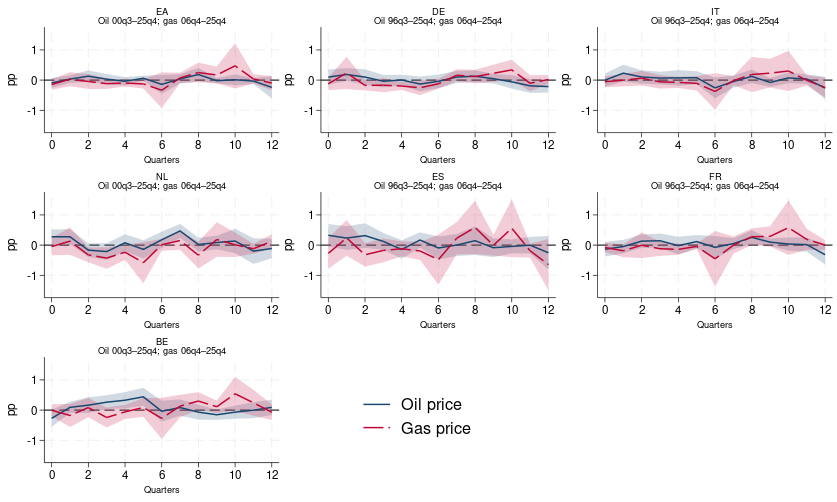
\includegraphics[width=1\textwidth]{lp_iv_og_ctry_wageH.png}
  \begin{minipage}{0.95\textwidth}\footnotesize
  \emph{Notes}: Response (percentage points) of year-on-year growth in gross wages per hour worked to a 10 percentage point increase in the year-on-year growth of the oil and natural gas prices; 90\% confidence bands. 2SLS local projections: the oil price change is instrumented with the three monthly Mori--Peersman oil supply news shocks of the quarter, the gas price change with the three monthly Alessandri--Gazzani gas supply shocks of the quarter. Time series for the euro area and for each country, Newey--West standard errors; same vertical scale in all panels; the sample (shock dates, $h=0$) for oil and gas is shown under each panel name. Controls (both stages): 4 lags of the outcome and of the price change, log industrial production, unemployment rate and 1-year Bund yield; COVID dummy 2020--2022. Sources: Eurostat (quarterly national accounts); Instruments: Mori and Peersman; Alessandri and Gazzani (2025). Eurostat and Bundesbank for the controls. Energy prices: quarterly averages of monthly data (file \texttt{Data\_OIL\_ELE\_GAS.xlsx}).
  \end{minipage}
\end{figure}

\clearpage

\begin{appendices}

%==============================================================================
\section{Labour market: oil and gas (IV)}
%==============================================================================

\subsection{Hours worked}

\noindent\textbf{Comment.} \tbc{reading of the IV responses of hours worked to oil and gas price shocks: sign, size, timing and persistence; differences between oil and gas and across countries; comparison with OLS (Appendix~\ref{app:ols})}.


\begin{figure}[H]
  \centering
  \caption{Oil and gas $\rightarrow$ hours worked: euro area}
  \label{fig:lp_iv_og_EA_occH}
  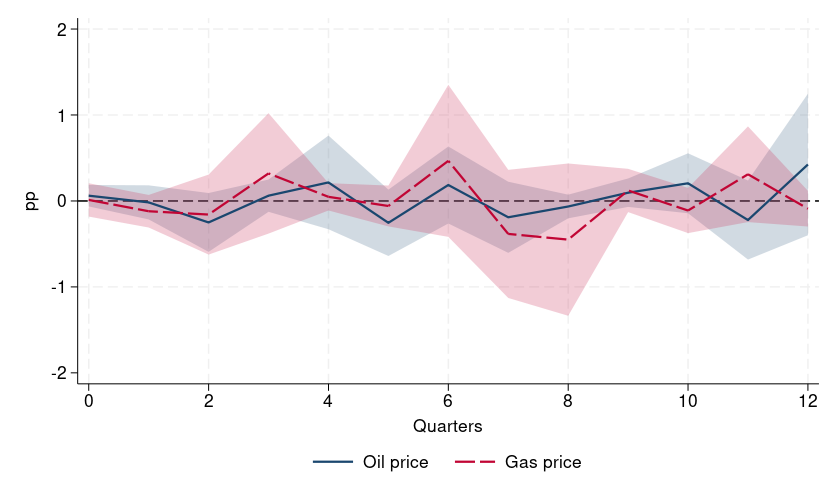
\includegraphics[width=0.7\textwidth]{lp_iv_og_EA_occH.png}
  \begin{minipage}{0.95\textwidth}\footnotesize
  \emph{Notes}: Response (percentage points) of quarter-on-quarter growth in hours worked (total economy) to a 10 percentage point increase in the year-on-year growth of the oil and natural gas prices; 90\% confidence bands. 2SLS local projections: the oil price change is instrumented with the three monthly Mori--Peersman oil supply news shocks of the quarter, the gas price change with the three monthly Alessandri--Gazzani gas supply shocks of the quarter. Time-series estimate for the euro area, Newey--West standard errors. Controls (both stages): 4 lags of the outcome and of the price change, log industrial production, unemployment rate and 1-year Bund yield; COVID dummy 2020--2022. Sample (shock dates, $h=0$): \smp{lp_iv_og_EA_occH}. Sources: Eurostat (quarterly national accounts); Instruments: Mori and Peersman; Alessandri and Gazzani (2025). Eurostat and Bundesbank for the controls. Energy prices: quarterly averages of monthly data (file \texttt{Data\_OIL\_ELE\_GAS.xlsx}).
  \end{minipage}
\end{figure}

\begin{figure}[H]
  \centering
  \caption{Oil and gas $\rightarrow$ hours worked: euro area and countries}
  \label{fig:lp_iv_og_ctry_occH}
  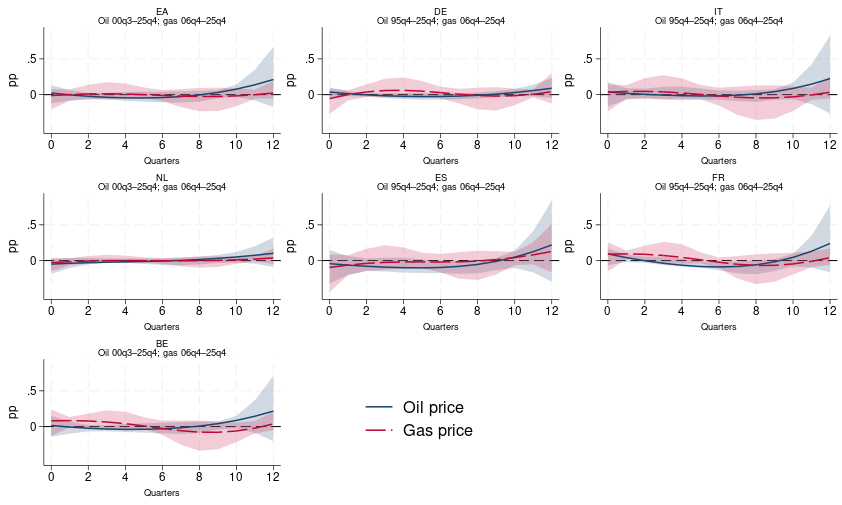
\includegraphics[width=1\textwidth]{lp_iv_og_ctry_occH.png}
  \begin{minipage}{0.95\textwidth}\footnotesize
  \emph{Notes}: Response (percentage points) of quarter-on-quarter growth in hours worked (total economy) to a 10 percentage point increase in the year-on-year growth of the oil and natural gas prices; 90\% confidence bands. 2SLS local projections: the oil price change is instrumented with the three monthly Mori--Peersman oil supply news shocks of the quarter, the gas price change with the three monthly Alessandri--Gazzani gas supply shocks of the quarter. Time series for the euro area and for each country, Newey--West standard errors; same vertical scale in all panels; the sample (shock dates, $h=0$) for oil and gas is shown under each panel name. Controls (both stages): 4 lags of the outcome and of the price change, log industrial production, unemployment rate and 1-year Bund yield; COVID dummy 2020--2022. Sources: Eurostat (quarterly national accounts); Instruments: Mori and Peersman; Alessandri and Gazzani (2025). Eurostat and Bundesbank for the controls. Energy prices: quarterly averages of monthly data (file \texttt{Data\_OIL\_ELE\_GAS.xlsx}).
  \end{minipage}
\end{figure}

\clearpage

\subsection{Unemployment rate}

\noindent\textbf{Comment.} \tbc{reading of the IV responses of unemployment rate to oil and gas price shocks: sign, size, timing and persistence; differences between oil and gas and across countries; comparison with OLS (Appendix~\ref{app:ols})}.


\begin{figure}[H]
  \centering
  \caption{Oil and gas $\rightarrow$ unemployment rate: euro area}
  \label{fig:lp_iv_og_EA_dur}
  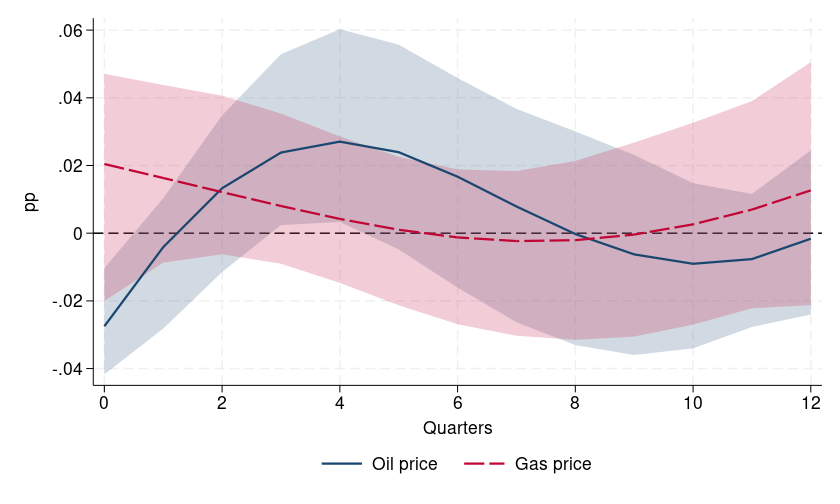
\includegraphics[width=0.7\textwidth]{lp_iv_og_EA_dur.png}
  \begin{minipage}{0.95\textwidth}\footnotesize
  \emph{Notes}: Response (percentage points) of the quarter-on-quarter change in the unemployment rate to a 10 percentage point increase in the year-on-year growth of the oil and natural gas prices; 90\% confidence bands. 2SLS local projections: the oil price change is instrumented with the three monthly Mori--Peersman oil supply news shocks of the quarter, the gas price change with the three monthly Alessandri--Gazzani gas supply shocks of the quarter. Time-series estimate for the euro area, Newey--West standard errors. Controls (both stages): 4 lags of the outcome and of the price change, log industrial production, 1-year Bund yield (the unemployment rate level is left out, as it is collinear with the lags of the outcome); COVID dummy 2020--2022. Sample (shock dates, $h=0$): \smp{lp_iv_og_EA_dur}. Sources: Eurostat (\texttt{une\_rt\_m}); Instruments: Mori and Peersman; Alessandri and Gazzani (2025). Eurostat and Bundesbank for the controls. Energy prices: quarterly averages of monthly data (file \texttt{Data\_OIL\_ELE\_GAS.xlsx}).
  \end{minipage}
\end{figure}

\begin{figure}[H]
  \centering
  \caption{Oil and gas $\rightarrow$ unemployment rate: euro area and countries}
  \label{fig:lp_iv_og_ctry_dur}
  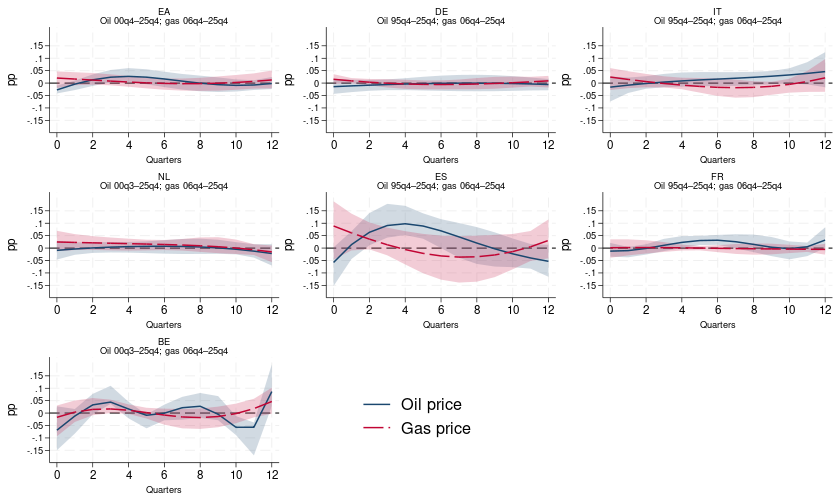
\includegraphics[width=1\textwidth]{lp_iv_og_ctry_dur.png}
  \begin{minipage}{0.95\textwidth}\footnotesize
  \emph{Notes}: Response (percentage points) of the quarter-on-quarter change in the unemployment rate to a 10 percentage point increase in the year-on-year growth of the oil and natural gas prices; 90\% confidence bands. 2SLS local projections: the oil price change is instrumented with the three monthly Mori--Peersman oil supply news shocks of the quarter, the gas price change with the three monthly Alessandri--Gazzani gas supply shocks of the quarter. Time series for the euro area and for each country, Newey--West standard errors; same vertical scale in all panels; the sample (shock dates, $h=0$) for oil and gas is shown under each panel name. Controls (both stages): 4 lags of the outcome and of the price change, log industrial production, 1-year Bund yield (the unemployment rate level is left out, as it is collinear with the lags of the outcome); COVID dummy 2020--2022. Sources: Eurostat (\texttt{une\_rt\_m}); Instruments: Mori and Peersman; Alessandri and Gazzani (2025). Eurostat and Bundesbank for the controls. Energy prices: quarterly averages of monthly data (file \texttt{Data\_OIL\_ELE\_GAS.xlsx}).
  \end{minipage}
\end{figure}

\clearpage

%==============================================================================
\section{IV robustness: quarterly-average instrument and pre-COVID sample}
%==============================================================================

\subsection{HICP}

\begin{figure}[H]
  \centering
  \caption{Oil $\rightarrow$ HICP: euro area, IV robustness}
  \label{fig:lp_iv_rob_OilSpotUSDBarrel_hicp}
  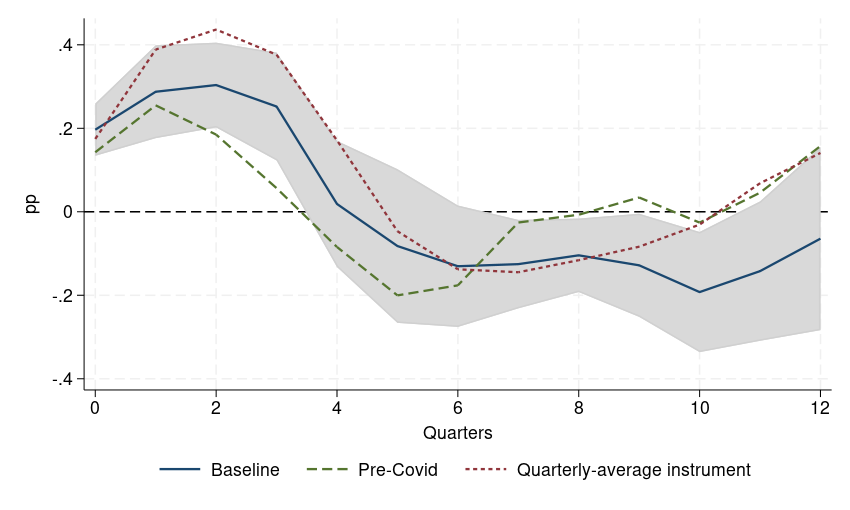
\includegraphics[width=0.7\textwidth]{lp_iv_rob_OilSpotUSDBarrel_hicp.png}
  \begin{minipage}{0.95\textwidth}\footnotesize
  \emph{Notes}: Response (percentage points) of year-on-year HICP inflation to a 10 percentage point increase in the year-on-year growth in the oil price (spot, USD per barrel). Euro area, time series, Newey--West standard errors. Baseline: 2SLS with the three monthly shocks of the quarter as instruments (90\% band). Pre-COVID: baseline on data before 2020q1 only ($t+h \le$ 2019q4), without the COVID dummy. Quarterly-average instrument: one instrument, the average of the three monthly shocks. Controls (both stages): 4 lags of the outcome and of the price change, log industrial production, unemployment rate and 1-year Bund yield; COVID dummy 2020--2022. Sources: Eurostat (HICP, \texttt{prc\_hicp\_midx}); Instruments: Mori and Peersman; Alessandri and Gazzani (2025). Eurostat and Bundesbank for the controls. Energy prices: quarterly averages of monthly data (file \texttt{Data\_OIL\_ELE\_GAS.xlsx}).
  \end{minipage}
\end{figure}

\begin{figure}[H]
  \centering
  \caption{Gas $\rightarrow$ HICP: euro area, IV robustness}
  \label{fig:lp_iv_rob_TTFSpotEURMWH_hicp}
  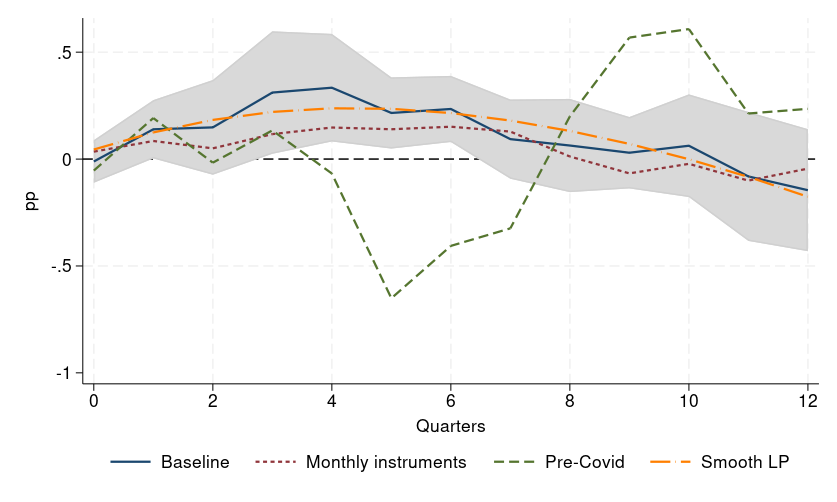
\includegraphics[width=0.7\textwidth]{lp_iv_rob_TTFSpotEURMWH_hicp.png}
  \begin{minipage}{0.95\textwidth}\footnotesize
  \emph{Notes}: Response (percentage points) of year-on-year HICP inflation to a 10 percentage point increase in the year-on-year growth in the natural gas price (TTF, EUR/MWh). Euro area, time series, Newey--West standard errors. Baseline: 2SLS with the three monthly shocks of the quarter as instruments (90\% band). Pre-COVID: baseline on data before 2020q1 only ($t+h \le$ 2019q4), without the COVID dummy. Quarterly-average instrument: one instrument, the average of the three monthly shocks. Controls (both stages): 4 lags of the outcome and of the price change, log industrial production, unemployment rate and 1-year Bund yield; COVID dummy 2020--2022. Sources: Eurostat (HICP, \texttt{prc\_hicp\_midx}); Instruments: Mori and Peersman; Alessandri and Gazzani (2025). Eurostat and Bundesbank for the controls. Energy prices: quarterly averages of monthly data (file \texttt{Data\_OIL\_ELE\_GAS.xlsx}).
  \end{minipage}
\end{figure}

\clearpage

\subsection{Negotiated wages}

\begin{figure}[H]
  \centering
  \caption{Oil $\rightarrow$ negotiated wages: euro area, IV robustness}
  \label{fig:lp_iv_rob_OilSpotUSDBarrel_contr}
  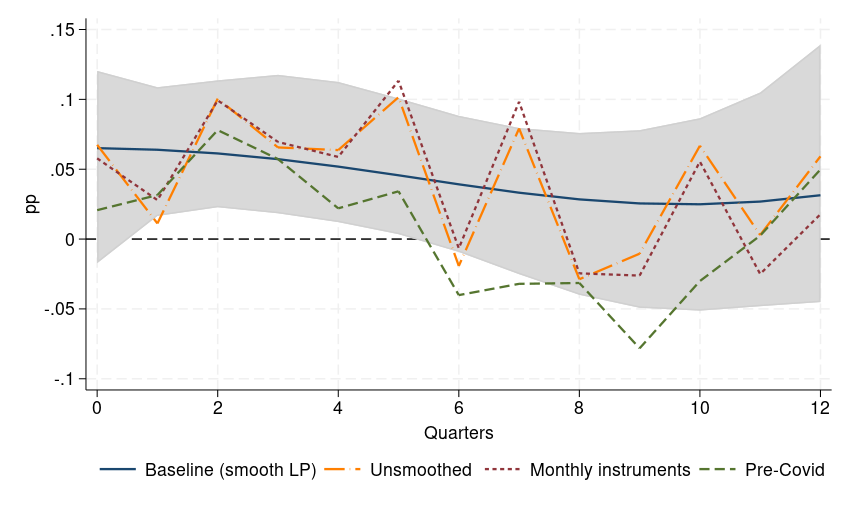
\includegraphics[width=0.7\textwidth]{lp_iv_rob_OilSpotUSDBarrel_contr.png}
  \begin{minipage}{0.95\textwidth}\footnotesize
  \emph{Notes}: Response (percentage points) of year-on-year negotiated wage growth to a 10 percentage point increase in the year-on-year growth in the oil price (spot, USD per barrel). Euro area, time series, Newey--West standard errors. Baseline: 2SLS with the three monthly shocks of the quarter as instruments (90\% band). Pre-COVID: baseline on data before 2020q1 only ($t+h \le$ 2019q4), without the COVID dummy. Quarterly-average instrument: one instrument, the average of the three monthly shocks. Controls (both stages): 4 lags of the outcome and of the price change, log industrial production, unemployment rate and 1-year Bund yield; COVID dummy 2020--2022. Sources: ECB (indicator of negotiated wage rates, INW); Instruments: Mori and Peersman; Alessandri and Gazzani (2025). Eurostat and Bundesbank for the controls. Energy prices: quarterly averages of monthly data (file \texttt{Data\_OIL\_ELE\_GAS.xlsx}).
  \end{minipage}
\end{figure}

\begin{figure}[H]
  \centering
  \caption{Gas $\rightarrow$ negotiated wages: euro area, IV robustness}
  \label{fig:lp_iv_rob_TTFSpotEURMWH_contr}
  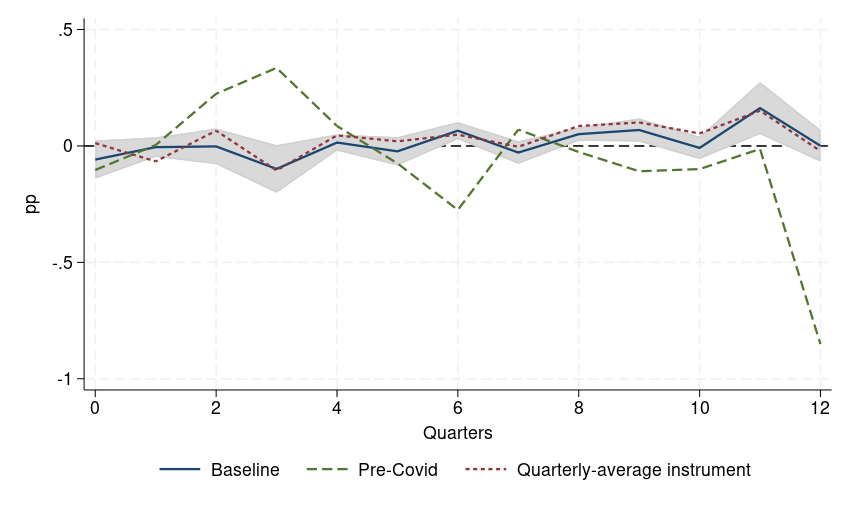
\includegraphics[width=0.7\textwidth]{lp_iv_rob_TTFSpotEURMWH_contr.png}
  \begin{minipage}{0.95\textwidth}\footnotesize
  \emph{Notes}: Response (percentage points) of year-on-year negotiated wage growth to a 10 percentage point increase in the year-on-year growth in the natural gas price (TTF, EUR/MWh). Euro area, time series, Newey--West standard errors. Baseline: 2SLS with the three monthly shocks of the quarter as instruments (90\% band). Pre-COVID: baseline on data before 2020q1 only ($t+h \le$ 2019q4), without the COVID dummy. Quarterly-average instrument: one instrument, the average of the three monthly shocks. Controls (both stages): 4 lags of the outcome and of the price change, log industrial production, unemployment rate and 1-year Bund yield; COVID dummy 2020--2022. Sources: ECB (indicator of negotiated wage rates, INW); Instruments: Mori and Peersman; Alessandri and Gazzani (2025). Eurostat and Bundesbank for the controls. Energy prices: quarterly averages of monthly data (file \texttt{Data\_OIL\_ELE\_GAS.xlsx}).
  \end{minipage}
\end{figure}

\clearpage

\subsection{Hourly wages}

\begin{figure}[H]
  \centering
  \caption{Oil $\rightarrow$ hourly wages: euro area, IV robustness}
  \label{fig:lp_iv_rob_OilSpotUSDBarrel_wageH}
  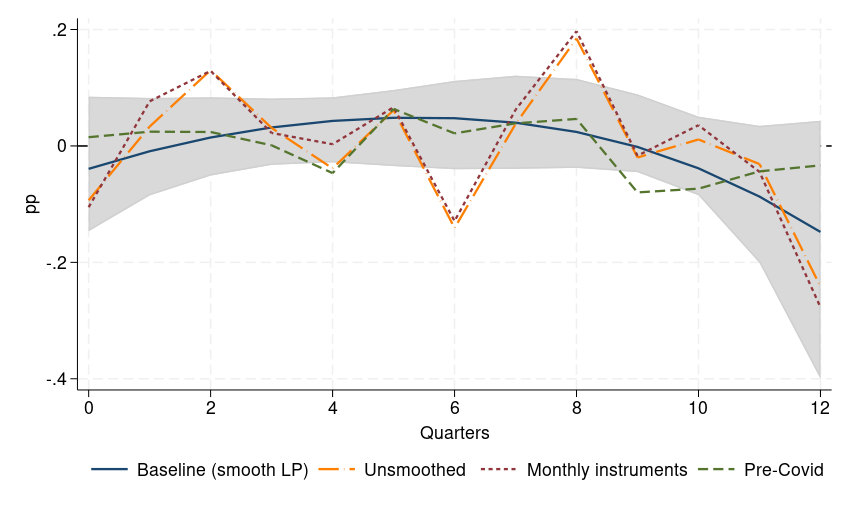
\includegraphics[width=0.7\textwidth]{lp_iv_rob_OilSpotUSDBarrel_wageH.png}
  \begin{minipage}{0.95\textwidth}\footnotesize
  \emph{Notes}: Response (percentage points) of year-on-year growth in gross wages per hour worked to a 10 percentage point increase in the year-on-year growth in the oil price (spot, USD per barrel). Euro area, time series, Newey--West standard errors. Baseline: 2SLS with the three monthly shocks of the quarter as instruments (90\% band). Pre-COVID: baseline on data before 2020q1 only ($t+h \le$ 2019q4), without the COVID dummy. Quarterly-average instrument: one instrument, the average of the three monthly shocks. Controls (both stages): 4 lags of the outcome and of the price change, log industrial production, unemployment rate and 1-year Bund yield; COVID dummy 2020--2022. Sources: Eurostat (quarterly national accounts); Instruments: Mori and Peersman; Alessandri and Gazzani (2025). Eurostat and Bundesbank for the controls. Energy prices: quarterly averages of monthly data (file \texttt{Data\_OIL\_ELE\_GAS.xlsx}).
  \end{minipage}
\end{figure}

\begin{figure}[H]
  \centering
  \caption{Gas $\rightarrow$ hourly wages: euro area, IV robustness}
  \label{fig:lp_iv_rob_TTFSpotEURMWH_wageH}
  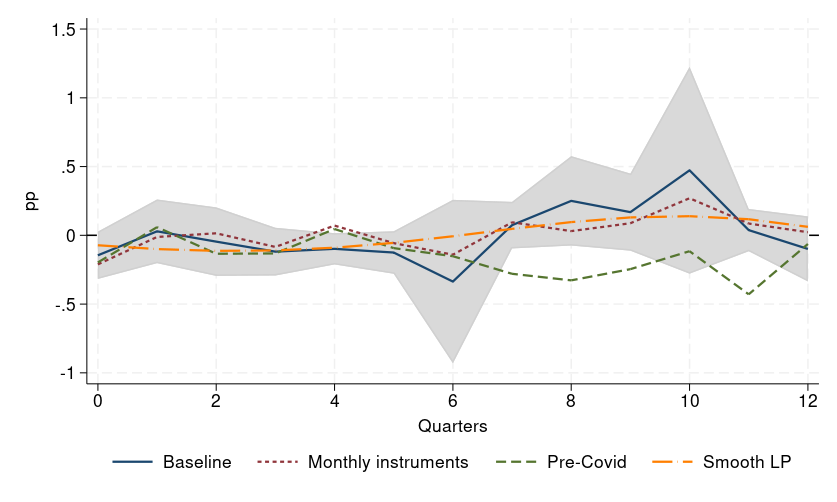
\includegraphics[width=0.7\textwidth]{lp_iv_rob_TTFSpotEURMWH_wageH.png}
  \begin{minipage}{0.95\textwidth}\footnotesize
  \emph{Notes}: Response (percentage points) of year-on-year growth in gross wages per hour worked to a 10 percentage point increase in the year-on-year growth in the natural gas price (TTF, EUR/MWh). Euro area, time series, Newey--West standard errors. Baseline: 2SLS with the three monthly shocks of the quarter as instruments (90\% band). Pre-COVID: baseline on data before 2020q1 only ($t+h \le$ 2019q4), without the COVID dummy. Quarterly-average instrument: one instrument, the average of the three monthly shocks. Controls (both stages): 4 lags of the outcome and of the price change, log industrial production, unemployment rate and 1-year Bund yield; COVID dummy 2020--2022. Sources: Eurostat (quarterly national accounts); Instruments: Mori and Peersman; Alessandri and Gazzani (2025). Eurostat and Bundesbank for the controls. Energy prices: quarterly averages of monthly data (file \texttt{Data\_OIL\_ELE\_GAS.xlsx}).
  \end{minipage}
\end{figure}

\clearpage

\subsection{Hours worked}

\begin{figure}[H]
  \centering
  \caption{Oil $\rightarrow$ hours worked: euro area, IV robustness}
  \label{fig:lp_iv_rob_OilSpotUSDBarrel_occH}
  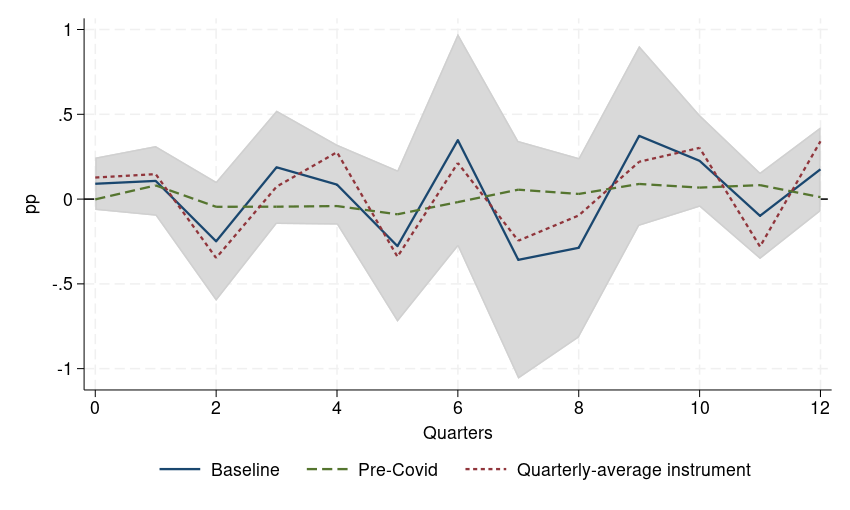
\includegraphics[width=0.7\textwidth]{lp_iv_rob_OilSpotUSDBarrel_occH.png}
  \begin{minipage}{0.95\textwidth}\footnotesize
  \emph{Notes}: Response (percentage points) of quarter-on-quarter growth in hours worked (total economy) to a 10 percentage point increase in the year-on-year growth in the oil price (spot, USD per barrel). Euro area, time series, Newey--West standard errors. Baseline: 2SLS with the three monthly shocks of the quarter as instruments (90\% band). Pre-COVID: baseline on data before 2020q1 only ($t+h \le$ 2019q4), without the COVID dummy. Quarterly-average instrument: one instrument, the average of the three monthly shocks. Controls (both stages): 4 lags of the outcome and of the price change, log industrial production, unemployment rate and 1-year Bund yield; COVID dummy 2020--2022. Sources: Eurostat (quarterly national accounts); Instruments: Mori and Peersman; Alessandri and Gazzani (2025). Eurostat and Bundesbank for the controls. Energy prices: quarterly averages of monthly data (file \texttt{Data\_OIL\_ELE\_GAS.xlsx}).
  \end{minipage}
\end{figure}

\begin{figure}[H]
  \centering
  \caption{Gas $\rightarrow$ hours worked: euro area, IV robustness}
  \label{fig:lp_iv_rob_TTFSpotEURMWH_occH}
  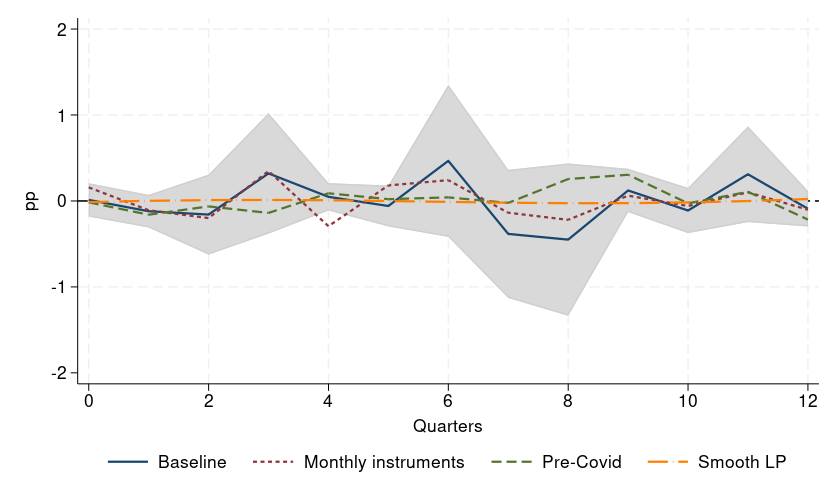
\includegraphics[width=0.7\textwidth]{lp_iv_rob_TTFSpotEURMWH_occH.png}
  \begin{minipage}{0.95\textwidth}\footnotesize
  \emph{Notes}: Response (percentage points) of quarter-on-quarter growth in hours worked (total economy) to a 10 percentage point increase in the year-on-year growth in the natural gas price (TTF, EUR/MWh). Euro area, time series, Newey--West standard errors. Baseline: 2SLS with the three monthly shocks of the quarter as instruments (90\% band). Pre-COVID: baseline on data before 2020q1 only ($t+h \le$ 2019q4), without the COVID dummy. Quarterly-average instrument: one instrument, the average of the three monthly shocks. Controls (both stages): 4 lags of the outcome and of the price change, log industrial production, unemployment rate and 1-year Bund yield; COVID dummy 2020--2022. Sources: Eurostat (quarterly national accounts); Instruments: Mori and Peersman; Alessandri and Gazzani (2025). Eurostat and Bundesbank for the controls. Energy prices: quarterly averages of monthly data (file \texttt{Data\_OIL\_ELE\_GAS.xlsx}).
  \end{minipage}
\end{figure}

\clearpage

\subsection{Unemployment rate}

\begin{figure}[H]
  \centering
  \caption{Oil $\rightarrow$ unemployment rate: euro area, IV robustness}
  \label{fig:lp_iv_rob_OilSpotUSDBarrel_dur}
  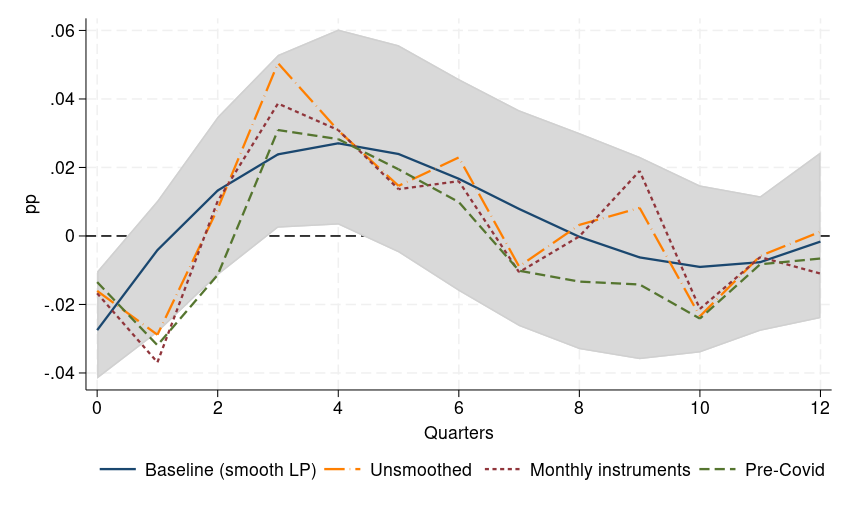
\includegraphics[width=0.7\textwidth]{lp_iv_rob_OilSpotUSDBarrel_dur.png}
  \begin{minipage}{0.95\textwidth}\footnotesize
  \emph{Notes}: Response (percentage points) of the quarter-on-quarter change in the unemployment rate to a 10 percentage point increase in the year-on-year growth in the oil price (spot, USD per barrel). Euro area, time series, Newey--West standard errors. Baseline: 2SLS with the three monthly shocks of the quarter as instruments (90\% band). Pre-COVID: baseline on data before 2020q1 only ($t+h \le$ 2019q4), without the COVID dummy. Quarterly-average instrument: one instrument, the average of the three monthly shocks. Controls (both stages): 4 lags of the outcome and of the price change, log industrial production, 1-year Bund yield (the unemployment rate level is left out, as it is collinear with the lags of the outcome); COVID dummy 2020--2022. Sources: Eurostat (\texttt{une\_rt\_m}); Instruments: Mori and Peersman; Alessandri and Gazzani (2025). Eurostat and Bundesbank for the controls. Energy prices: quarterly averages of monthly data (file \texttt{Data\_OIL\_ELE\_GAS.xlsx}).
  \end{minipage}
\end{figure}

\begin{figure}[H]
  \centering
  \caption{Gas $\rightarrow$ unemployment rate: euro area, IV robustness}
  \label{fig:lp_iv_rob_TTFSpotEURMWH_dur}
  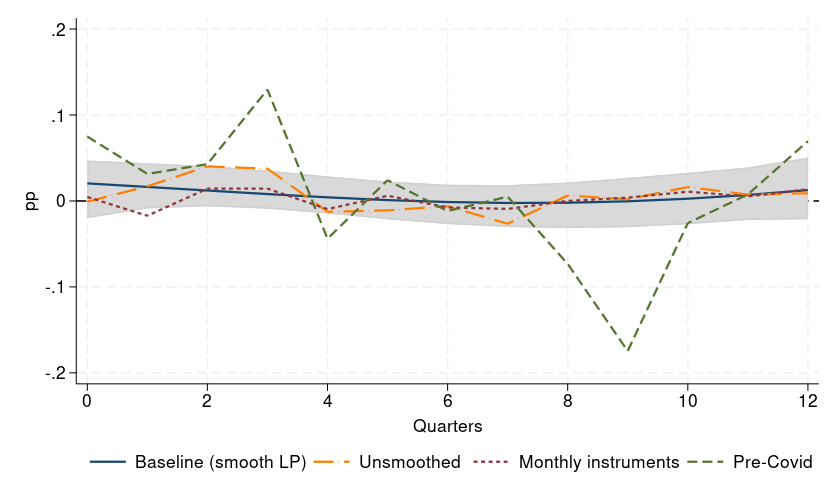
\includegraphics[width=0.7\textwidth]{lp_iv_rob_TTFSpotEURMWH_dur.png}
  \begin{minipage}{0.95\textwidth}\footnotesize
  \emph{Notes}: Response (percentage points) of the quarter-on-quarter change in the unemployment rate to a 10 percentage point increase in the year-on-year growth in the natural gas price (TTF, EUR/MWh). Euro area, time series, Newey--West standard errors. Baseline: 2SLS with the three monthly shocks of the quarter as instruments (90\% band). Pre-COVID: baseline on data before 2020q1 only ($t+h \le$ 2019q4), without the COVID dummy. Quarterly-average instrument: one instrument, the average of the three monthly shocks. Controls (both stages): 4 lags of the outcome and of the price change, log industrial production, 1-year Bund yield (the unemployment rate level is left out, as it is collinear with the lags of the outcome); COVID dummy 2020--2022. Sources: Eurostat (\texttt{une\_rt\_m}); Instruments: Mori and Peersman; Alessandri and Gazzani (2025). Eurostat and Bundesbank for the controls. Energy prices: quarterly averages of monthly data (file \texttt{Data\_OIL\_ELE\_GAS.xlsx}).
  \end{minipage}
\end{figure}

\clearpage

%==============================================================================
\section{OLS local projections}\label{app:ols}
%==============================================================================

\noindent Graphs from the last OLS run of \texttt{an\_lp\_energy\_ea.do} (switched off in
\texttt{master.do}).

\subsection{Consumer prices}

\begin{figure}[H]
  \centering
  \caption{Oil and gas $\rightarrow$ HICP: euro area, OLS}
  \label{fig:lp_og_EA_hicp}
  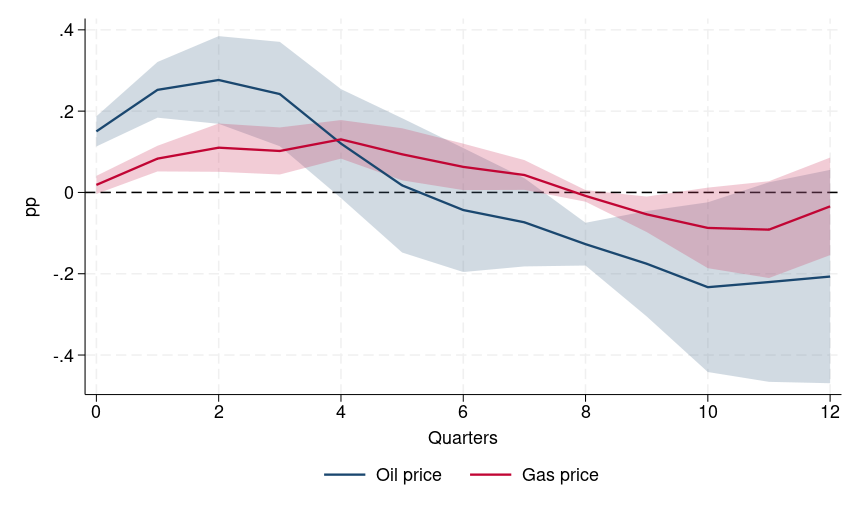
\includegraphics[width=0.7\textwidth]{lp_og_EA_hicp.png}
  \begin{minipage}{0.95\textwidth}\footnotesize
  \emph{Notes}: Response (percentage points) of year-on-year HICP inflation to a 10 percentage point increase in the year-on-year growth of the oil and natural gas prices; 90\% confidence bands. OLS local projections (the price change is not instrumented). Time-series estimate for the euro area, Newey--West standard errors. Controls (both stages): 4 lags of the outcome and of the price change, log industrial production, unemployment rate and 1-year Bund yield; COVID dummy 2020--2022. Sample (shock dates, $h=0$): \smp{lp_og_EA_hicp}. Sources: Eurostat (HICP, \texttt{prc\_hicp\_midx}); Eurostat and Bundesbank for the controls. Energy prices: quarterly averages of monthly data (file \texttt{Data\_OIL\_ELE\_GAS.xlsx}).
  \end{minipage}
\end{figure}

\begin{figure}[H]
  \centering
  \caption{Oil and gas $\rightarrow$ HICP: euro area and countries, OLS}
  \label{fig:lp_og_ctry_hicp}
  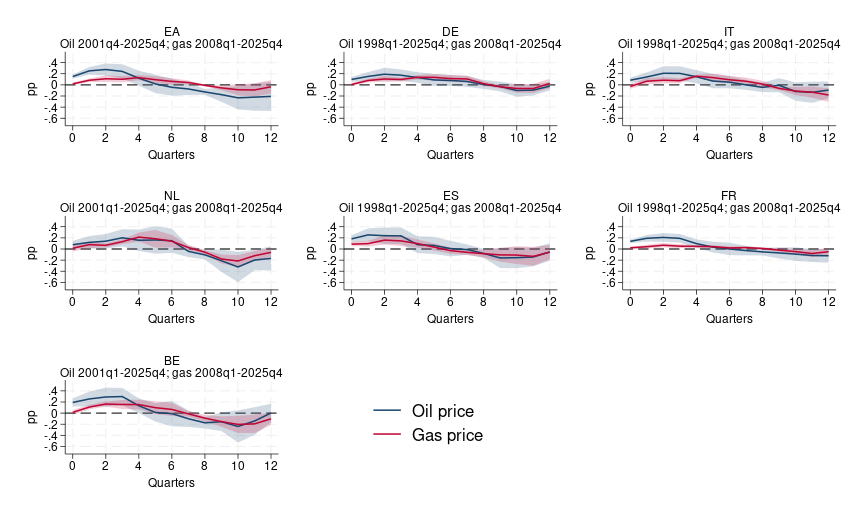
\includegraphics[width=1\textwidth]{lp_og_ctry_hicp.png}
  \begin{minipage}{0.95\textwidth}\footnotesize
  \emph{Notes}: Response (percentage points) of year-on-year HICP inflation to a 10 percentage point increase in the year-on-year growth of the oil and natural gas prices; 90\% confidence bands. OLS local projections (the price change is not instrumented). Time series for the euro area and for each country, Newey--West standard errors; same vertical scale in all panels; the sample (shock dates, $h=0$) for oil and gas is shown under each panel name. Controls (both stages): 4 lags of the outcome and of the price change, log industrial production, unemployment rate and 1-year Bund yield; COVID dummy 2020--2022. Sources: Eurostat (HICP, \texttt{prc\_hicp\_midx}); Eurostat and Bundesbank for the controls. Energy prices: quarterly averages of monthly data (file \texttt{Data\_OIL\_ELE\_GAS.xlsx}).
  \end{minipage}
\end{figure}

\clearpage

\subsection{Negotiated wages}

\begin{figure}[H]
  \centering
  \caption{Oil and gas $\rightarrow$ negotiated wages: euro area, OLS}
  \label{fig:lp_og_EA_contr}
  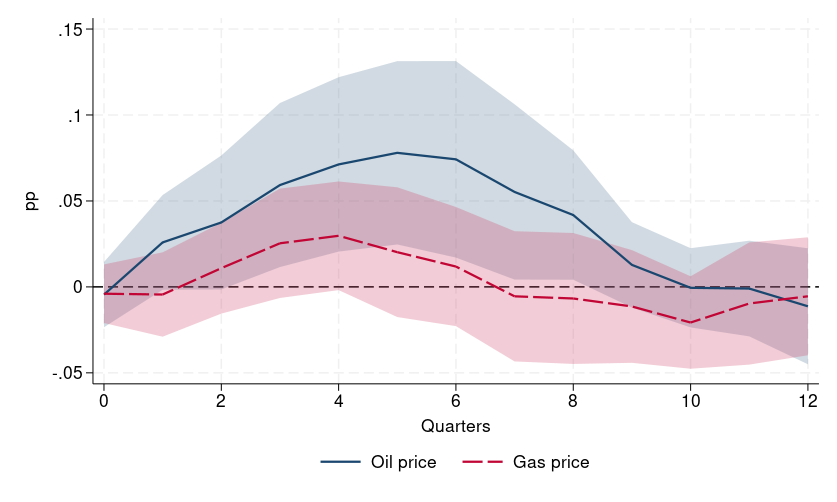
\includegraphics[width=0.7\textwidth]{lp_og_EA_contr.png}
  \begin{minipage}{0.95\textwidth}\footnotesize
  \emph{Notes}: Response (percentage points) of year-on-year negotiated wage growth to a 10 percentage point increase in the year-on-year growth of the oil and natural gas prices; 90\% confidence bands. OLS local projections (the price change is not instrumented). Time-series estimate for the euro area, Newey--West standard errors. Controls (both stages): 4 lags of the outcome and of the price change, log industrial production, unemployment rate and 1-year Bund yield; COVID dummy 2020--2022. Sample (shock dates, $h=0$): \smp{lp_og_EA_contr}. Sources: ECB (indicator of negotiated wage rates, INW); Eurostat and Bundesbank for the controls. Energy prices: quarterly averages of monthly data (file \texttt{Data\_OIL\_ELE\_GAS.xlsx}).
  \end{minipage}
\end{figure}

\begin{figure}[H]
  \centering
  \caption{Oil and gas $\rightarrow$ negotiated wages: euro area and countries, OLS}
  \label{fig:lp_og_ctry_contr}
  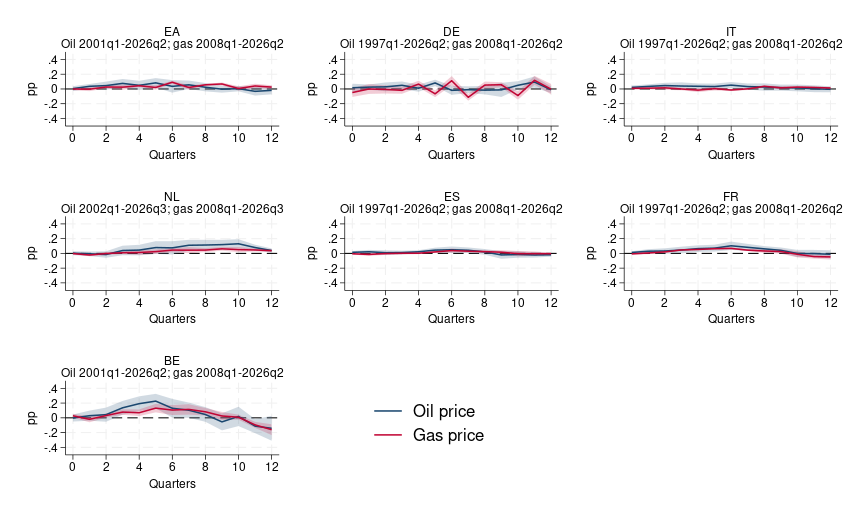
\includegraphics[width=1\textwidth]{lp_og_ctry_contr.png}
  \begin{minipage}{0.95\textwidth}\footnotesize
  \emph{Notes}: Response (percentage points) of year-on-year negotiated wage growth to a 10 percentage point increase in the year-on-year growth of the oil and natural gas prices; 90\% confidence bands. OLS local projections (the price change is not instrumented). Time series for the euro area and for each country, Newey--West standard errors; same vertical scale in all panels; the sample (shock dates, $h=0$) for oil and gas is shown under each panel name. Controls (both stages): 4 lags of the outcome and of the price change, log industrial production, unemployment rate and 1-year Bund yield; COVID dummy 2020--2022. Sources: ECB (indicator of negotiated wage rates, INW); Eurostat and Bundesbank for the controls. Energy prices: quarterly averages of monthly data (file \texttt{Data\_OIL\_ELE\_GAS.xlsx}).
  \end{minipage}
\end{figure}

\clearpage

\subsection{National accounts wages}

\begin{figure}[H]
  \centering
  \caption{Oil and gas $\rightarrow$ hourly wages: euro area, OLS}
  \label{fig:lp_og_EA_wageH}
  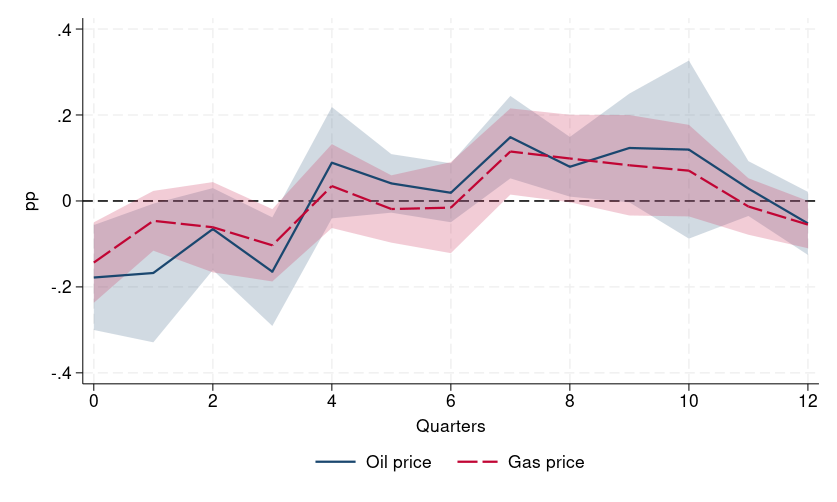
\includegraphics[width=0.7\textwidth]{lp_og_EA_wageH.png}
  \begin{minipage}{0.95\textwidth}\footnotesize
  \emph{Notes}: Response (percentage points) of year-on-year growth in gross wages per hour worked to a 10 percentage point increase in the year-on-year growth of the oil and natural gas prices; 90\% confidence bands. OLS local projections (the price change is not instrumented). Time-series estimate for the euro area, Newey--West standard errors. Controls (both stages): 4 lags of the outcome and of the price change, log industrial production, unemployment rate and 1-year Bund yield; COVID dummy 2020--2022. Sample (shock dates, $h=0$): \smp{lp_og_EA_wageH}. Sources: Eurostat (quarterly national accounts); Eurostat and Bundesbank for the controls. Energy prices: quarterly averages of monthly data (file \texttt{Data\_OIL\_ELE\_GAS.xlsx}).
  \end{minipage}
\end{figure}

\begin{figure}[H]
  \centering
  \caption{Oil and gas $\rightarrow$ hourly wages: euro area and countries, OLS}
  \label{fig:lp_og_ctry_wageH}
  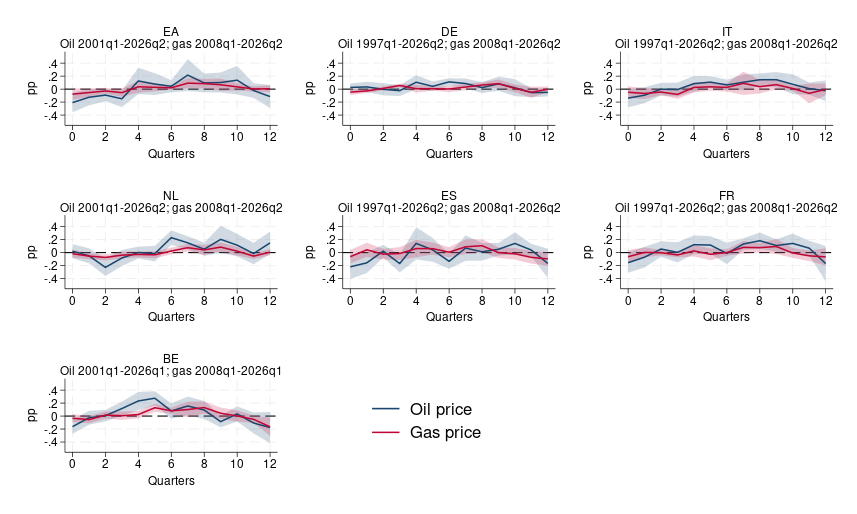
\includegraphics[width=1\textwidth]{lp_og_ctry_wageH.png}
  \begin{minipage}{0.95\textwidth}\footnotesize
  \emph{Notes}: Response (percentage points) of year-on-year growth in gross wages per hour worked to a 10 percentage point increase in the year-on-year growth of the oil and natural gas prices; 90\% confidence bands. OLS local projections (the price change is not instrumented). Time series for the euro area and for each country, Newey--West standard errors; same vertical scale in all panels; the sample (shock dates, $h=0$) for oil and gas is shown under each panel name. Controls (both stages): 4 lags of the outcome and of the price change, log industrial production, unemployment rate and 1-year Bund yield; COVID dummy 2020--2022. Sources: Eurostat (quarterly national accounts); Eurostat and Bundesbank for the controls. Energy prices: quarterly averages of monthly data (file \texttt{Data\_OIL\_ELE\_GAS.xlsx}).
  \end{minipage}
\end{figure}

\clearpage

\subsection{Hours worked}

\begin{figure}[H]
  \centering
  \caption{Oil and gas $\rightarrow$ hours worked: euro area, OLS}
  \label{fig:lp_og_EA_occH}
  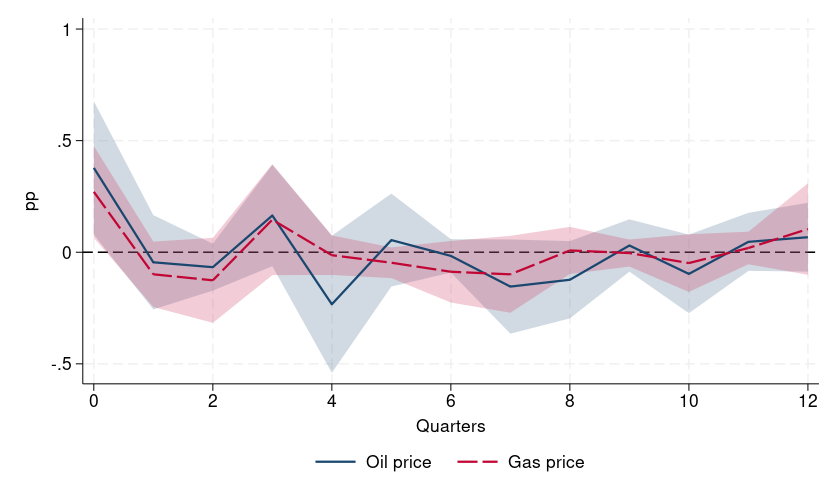
\includegraphics[width=0.7\textwidth]{lp_og_EA_occH.png}
  \begin{minipage}{0.95\textwidth}\footnotesize
  \emph{Notes}: Response (percentage points) of quarter-on-quarter growth in hours worked (total economy) to a 10 percentage point increase in the year-on-year growth of the oil and natural gas prices; 90\% confidence bands. OLS local projections (the price change is not instrumented). Time-series estimate for the euro area, Newey--West standard errors. Controls (both stages): 4 lags of the outcome and of the price change, log industrial production, unemployment rate and 1-year Bund yield; COVID dummy 2020--2022. Sample (shock dates, $h=0$): \smp{lp_og_EA_occH}. Sources: Eurostat (quarterly national accounts); Eurostat and Bundesbank for the controls. Energy prices: quarterly averages of monthly data (file \texttt{Data\_OIL\_ELE\_GAS.xlsx}).
  \end{minipage}
\end{figure}

\begin{figure}[H]
  \centering
  \caption{Oil and gas $\rightarrow$ hours worked: euro area and countries, OLS}
  \label{fig:lp_og_ctry_occH}
  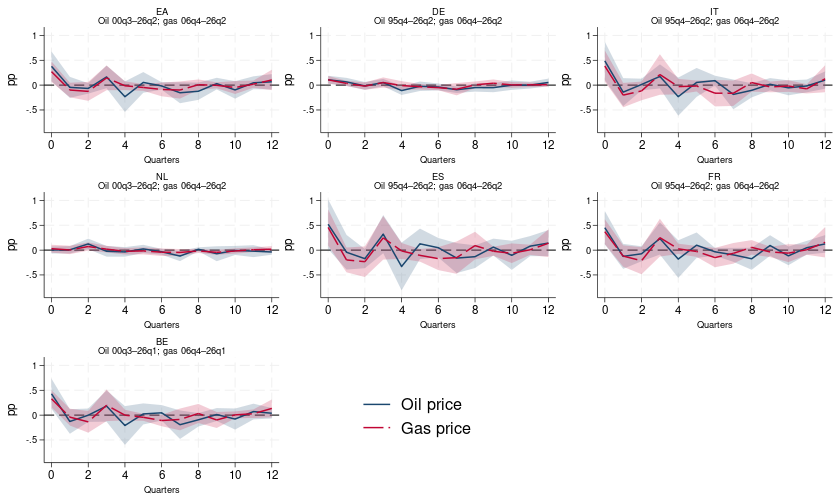
\includegraphics[width=1\textwidth]{lp_og_ctry_occH.png}
  \begin{minipage}{0.95\textwidth}\footnotesize
  \emph{Notes}: Response (percentage points) of quarter-on-quarter growth in hours worked (total economy) to a 10 percentage point increase in the year-on-year growth of the oil and natural gas prices; 90\% confidence bands. OLS local projections (the price change is not instrumented). Time series for the euro area and for each country, Newey--West standard errors; same vertical scale in all panels; the sample (shock dates, $h=0$) for oil and gas is shown under each panel name. Controls (both stages): 4 lags of the outcome and of the price change, log industrial production, unemployment rate and 1-year Bund yield; COVID dummy 2020--2022. Sources: Eurostat (quarterly national accounts); Eurostat and Bundesbank for the controls. Energy prices: quarterly averages of monthly data (file \texttt{Data\_OIL\_ELE\_GAS.xlsx}).
  \end{minipage}
\end{figure}

\clearpage

\subsection{Unemployment rate}

\begin{figure}[H]
  \centering
  \caption{Oil and gas $\rightarrow$ unemployment rate: euro area, OLS}
  \label{fig:lp_og_EA_dur}
  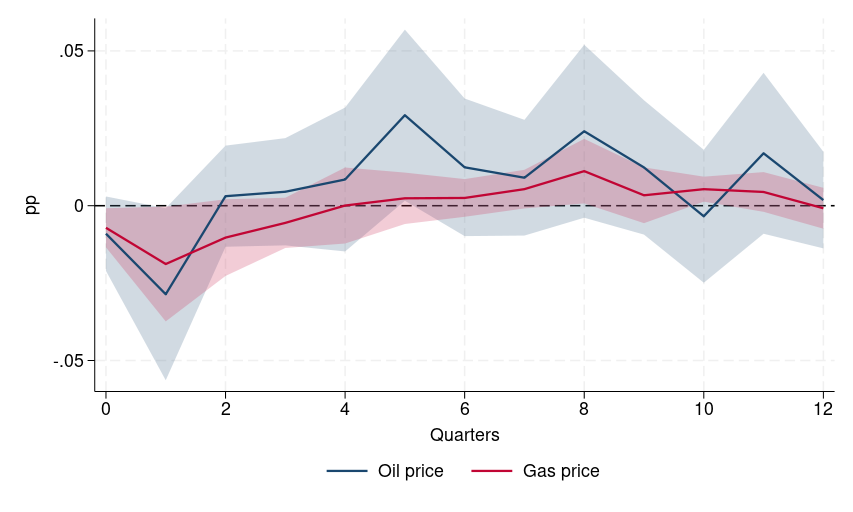
\includegraphics[width=0.7\textwidth]{lp_og_EA_dur.png}
  \begin{minipage}{0.95\textwidth}\footnotesize
  \emph{Notes}: Response (percentage points) of the quarter-on-quarter change in the unemployment rate to a 10 percentage point increase in the year-on-year growth of the oil and natural gas prices; 90\% confidence bands. OLS local projections (the price change is not instrumented). Time-series estimate for the euro area, Newey--West standard errors. Controls (both stages): 4 lags of the outcome and of the price change, log industrial production, 1-year Bund yield (the unemployment rate level is left out, as it is collinear with the lags of the outcome); COVID dummy 2020--2022. Sample (shock dates, $h=0$): \smp{lp_og_EA_dur}. Sources: Eurostat (\texttt{une\_rt\_m}); Eurostat and Bundesbank for the controls. Energy prices: quarterly averages of monthly data (file \texttt{Data\_OIL\_ELE\_GAS.xlsx}).
  \end{minipage}
\end{figure}

\begin{figure}[H]
  \centering
  \caption{Oil and gas $\rightarrow$ unemployment rate: euro area and countries, OLS}
  \label{fig:lp_og_ctry_dur}
  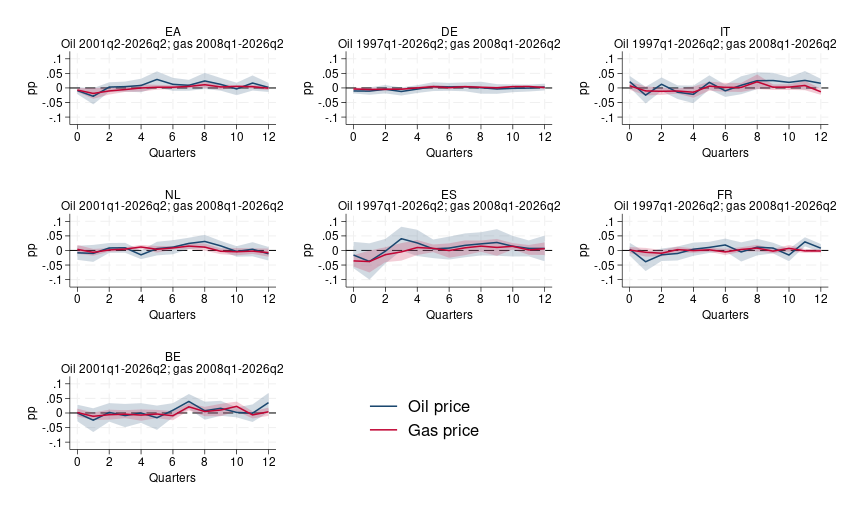
\includegraphics[width=1\textwidth]{lp_og_ctry_dur.png}
  \begin{minipage}{0.95\textwidth}\footnotesize
  \emph{Notes}: Response (percentage points) of the quarter-on-quarter change in the unemployment rate to a 10 percentage point increase in the year-on-year growth of the oil and natural gas prices; 90\% confidence bands. OLS local projections (the price change is not instrumented). Time series for the euro area and for each country, Newey--West standard errors; same vertical scale in all panels; the sample (shock dates, $h=0$) for oil and gas is shown under each panel name. Controls (both stages): 4 lags of the outcome and of the price change, log industrial production, 1-year Bund yield (the unemployment rate level is left out, as it is collinear with the lags of the outcome); COVID dummy 2020--2022. Sources: Eurostat (\texttt{une\_rt\_m}); Eurostat and Bundesbank for the controls. Energy prices: quarterly averages of monthly data (file \texttt{Data\_OIL\_ELE\_GAS.xlsx}).
  \end{minipage}
\end{figure}

\clearpage
\subsection{Electricity (OLS only)}

\begin{figure}[H]
  \centering
  \caption{Electricity $\rightarrow$ HICP: country panel, OLS}
  \label{fig:lp_main_ELEEURMWH_hicp}
  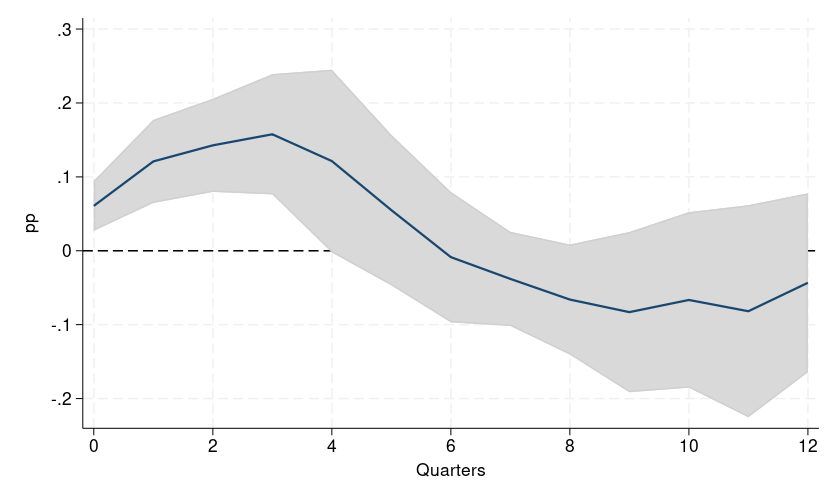
\includegraphics[width=0.7\textwidth]{lp_main_ELEEURMWH_hicp.png}
  \begin{minipage}{0.95\textwidth}\footnotesize
  \emph{Notes}: Response (percentage points) of year-on-year HICP inflation to a 10 percentage point increase in the year-on-year growth in the wholesale electricity price (EUR/MWh, national price). OLS panel estimate on DE, IT, NL, ES, FR (BE excluded: no electricity price), country fixed effects, weighted by average country employment, Driscoll--Kraay standard errors; no instrument is available for electricity. Controls (both stages): 4 lags of the outcome and of the price change, log industrial production, unemployment rate and 1-year Bund yield; COVID dummy 2020--2022. 90\% confidence band. Sample (shock dates, $h=0$): \smp{lp_main_ELEEURMWH_hicp}. Sources: Eurostat (HICP, \texttt{prc\_hicp\_midx}); Eurostat and Bundesbank for the controls. Energy prices: quarterly averages of monthly data (file \texttt{Data\_OIL\_ELE\_GAS.xlsx}).
  \end{minipage}
\end{figure}

\begin{figure}[H]
  \centering
  \caption{Electricity $\rightarrow$ negotiated wages: country panel, OLS}
  \label{fig:lp_main_ELEEURMWH_contr}
  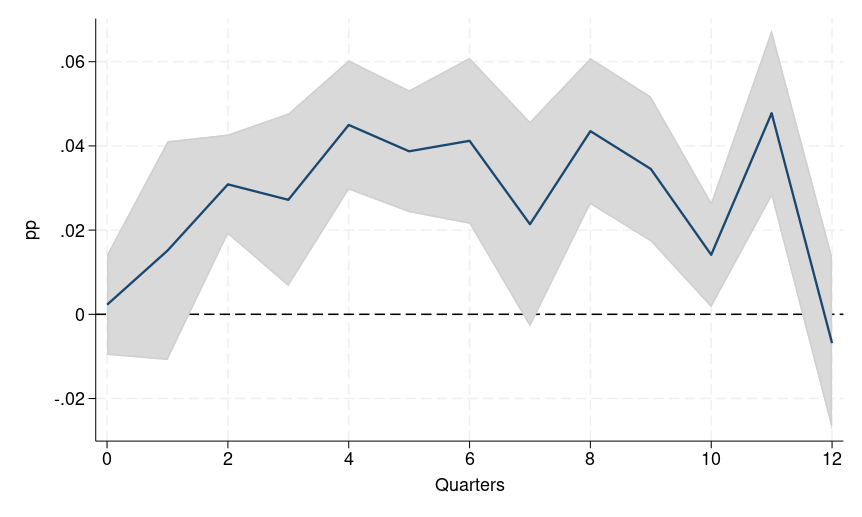
\includegraphics[width=0.7\textwidth]{lp_main_ELEEURMWH_contr.png}
  \begin{minipage}{0.95\textwidth}\footnotesize
  \emph{Notes}: Response (percentage points) of year-on-year negotiated wage growth to a 10 percentage point increase in the year-on-year growth in the wholesale electricity price (EUR/MWh, national price). OLS panel estimate on DE, IT, NL, ES, FR (BE excluded: no electricity price), country fixed effects, weighted by average country employment, Driscoll--Kraay standard errors; no instrument is available for electricity. Controls (both stages): 4 lags of the outcome and of the price change, log industrial production, unemployment rate and 1-year Bund yield; COVID dummy 2020--2022. 90\% confidence band. Sample (shock dates, $h=0$): \smp{lp_main_ELEEURMWH_contr}. Sources: ECB (indicator of negotiated wage rates, INW); Eurostat and Bundesbank for the controls. Energy prices: quarterly averages of monthly data (file \texttt{Data\_OIL\_ELE\_GAS.xlsx}).
  \end{minipage}
\end{figure}

\begin{figure}[H]
  \centering
  \caption{Electricity $\rightarrow$ hourly wages: country panel, OLS}
  \label{fig:lp_main_ELEEURMWH_wageH}
  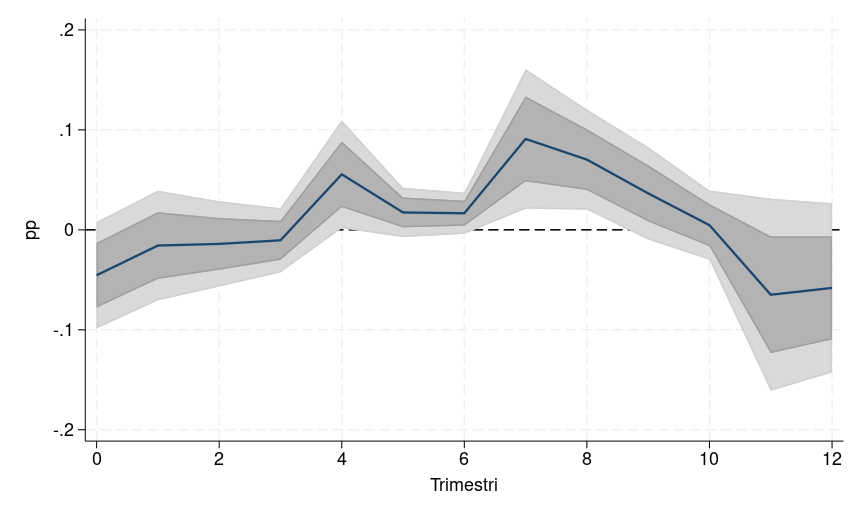
\includegraphics[width=0.7\textwidth]{lp_main_ELEEURMWH_wageH.png}
  \begin{minipage}{0.95\textwidth}\footnotesize
  \emph{Notes}: Response (percentage points) of year-on-year growth in gross wages per hour worked to a 10 percentage point increase in the year-on-year growth in the wholesale electricity price (EUR/MWh, national price). OLS panel estimate on DE, IT, NL, ES, FR (BE excluded: no electricity price), country fixed effects, weighted by average country employment, Driscoll--Kraay standard errors; no instrument is available for electricity. Controls (both stages): 4 lags of the outcome and of the price change, log industrial production, unemployment rate and 1-year Bund yield; COVID dummy 2020--2022. 90\% confidence band. Sample (shock dates, $h=0$): \smp{lp_main_ELEEURMWH_wageH}. Sources: Eurostat (quarterly national accounts); Eurostat and Bundesbank for the controls. Energy prices: quarterly averages of monthly data (file \texttt{Data\_OIL\_ELE\_GAS.xlsx}).
  \end{minipage}
\end{figure}

\begin{figure}[H]
  \centering
  \caption{Electricity $\rightarrow$ hours worked: country panel, OLS}
  \label{fig:lp_main_ELEEURMWH_occH}
  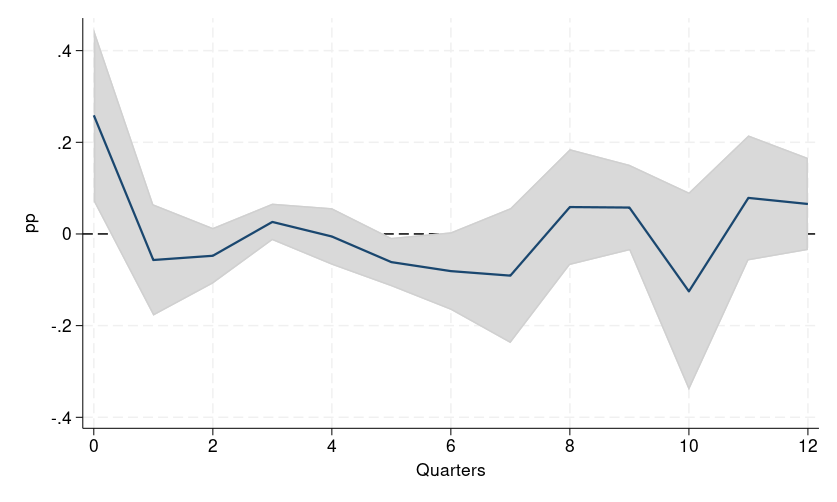
\includegraphics[width=0.7\textwidth]{lp_main_ELEEURMWH_occH.png}
  \begin{minipage}{0.95\textwidth}\footnotesize
  \emph{Notes}: Response (percentage points) of quarter-on-quarter growth in hours worked (total economy) to a 10 percentage point increase in the year-on-year growth in the wholesale electricity price (EUR/MWh, national price). OLS panel estimate on DE, IT, NL, ES, FR (BE excluded: no electricity price), country fixed effects, weighted by average country employment, Driscoll--Kraay standard errors; no instrument is available for electricity. Controls (both stages): 4 lags of the outcome and of the price change, log industrial production, unemployment rate and 1-year Bund yield; COVID dummy 2020--2022. 90\% confidence band. Sample (shock dates, $h=0$): \smp{lp_main_ELEEURMWH_occH}. Sources: Eurostat (quarterly national accounts); Eurostat and Bundesbank for the controls. Energy prices: quarterly averages of monthly data (file \texttt{Data\_OIL\_ELE\_GAS.xlsx}).
  \end{minipage}
\end{figure}

\begin{figure}[H]
  \centering
  \caption{Electricity $\rightarrow$ unemployment rate: country panel, OLS}
  \label{fig:lp_main_ELEEURMWH_dur}
  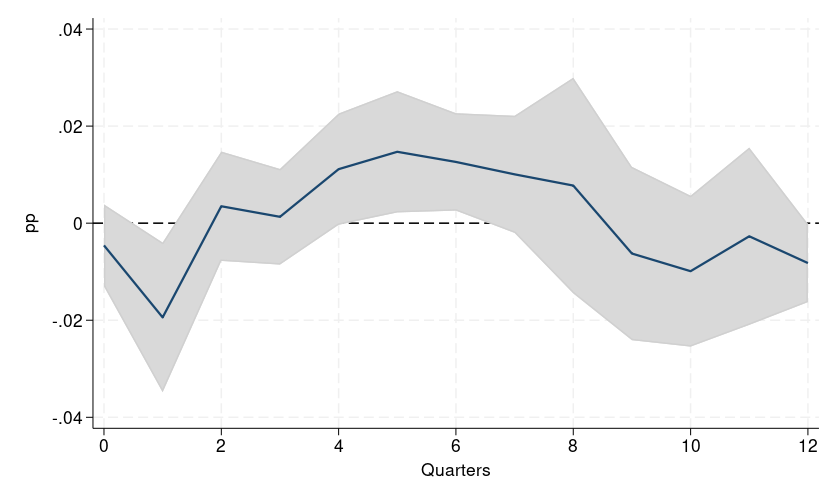
\includegraphics[width=0.7\textwidth]{lp_main_ELEEURMWH_dur.png}
  \begin{minipage}{0.95\textwidth}\footnotesize
  \emph{Notes}: Response (percentage points) of the quarter-on-quarter change in the unemployment rate to a 10 percentage point increase in the year-on-year growth in the wholesale electricity price (EUR/MWh, national price). OLS panel estimate on DE, IT, NL, ES, FR (BE excluded: no electricity price), country fixed effects, weighted by average country employment, Driscoll--Kraay standard errors; no instrument is available for electricity. Controls (both stages): 4 lags of the outcome and of the price change, log industrial production, 1-year Bund yield (the unemployment rate level is left out, as it is collinear with the lags of the outcome); COVID dummy 2020--2022. 90\% confidence band. Sample (shock dates, $h=0$): \smp{lp_main_ELEEURMWH_dur}. Sources: Eurostat (\texttt{une\_rt\_m}); Eurostat and Bundesbank for the controls. Energy prices: quarterly averages of monthly data (file \texttt{Data\_OIL\_ELE\_GAS.xlsx}).
  \end{minipage}
\end{figure}

\clearpage

\end{appendices}

\end{document}
